\section{Full Kitaev Triangle}

\begin{figure}[here]
  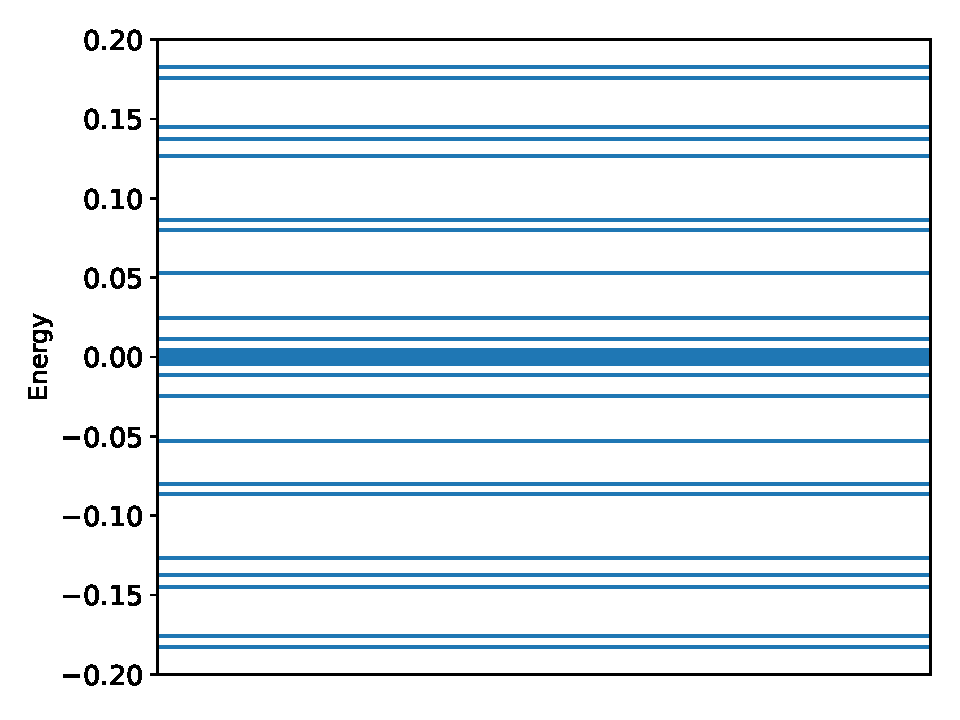
\includegraphics[0.3=\textwidth]{full-triangle-spectral-flow.pdf}
  \caption{Full trianglular island with length $L=25$ with a staggered vector potential described by Eq. \ref{eq:Heaviside-vector-potential}}
  \label{fig:full-triangle-energy}
\end{figure}


A quick note on why we use hollow triangular islands.
With the above gauge potentials present upon an equilateral triangle of arbitary length MZMs host at two of the corners and there live many edge states with in the band gap.
This energy spectra can be seen in Fig. \ref{fig:full-triangle-energy}, there appear to be many edge states near the zero-energy states.
We would like to use hollow triangular islands instead for two reasons: (1) $W \ll L$ is required for bulk-edge correspondence based on 1D topology to hold; (2) A finite $W$ is needed to gap out the chiral edge states of a 2D spinless \textit{p}-wave superconductor, i.e.\ opens a clean gap for the MZMs to host and braid in.

